\subsubsection{Component Diagram}
\begin{figure}[H]
	\centering
	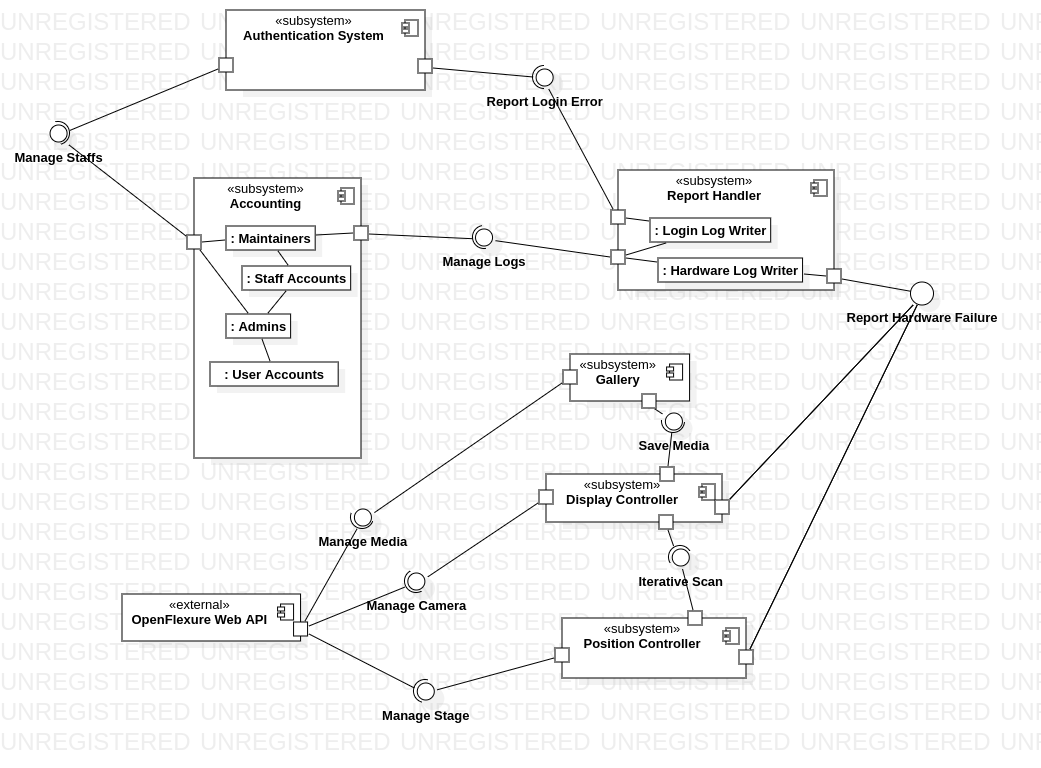
\includegraphics[scale=0.4]{Uml_Images/component_diagram}
	\caption{Component Diagram for OpenFlexure}
	\label{fig:component_diagram}
\end{figure}

\subsubsection{Deployment Diagram}
\begin{figure}[H]
	\centering
	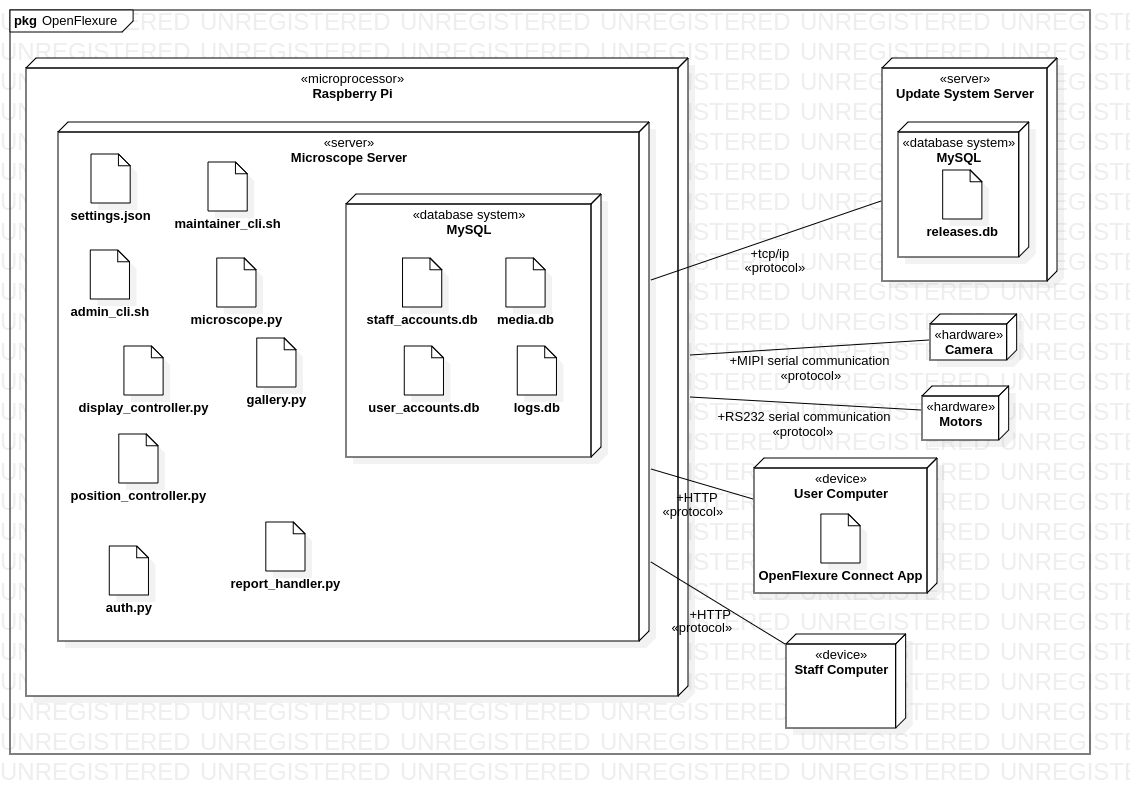
\includegraphics[scale=0.4]{Uml_Images/deployment_diagram}
	\caption{Deployment Diagram for OpenFlexure}
	\label{fig:deployment_diagram}
\end{figure}

\subsubsection{Design Rationale}
\paragraph{Component Diagram}
\begin{itemize}
	\item To allow the admins to use Block User and Unblock User functions defined in use-case diagram, Admins part is associated with the User Accounts part.
	\item To allow the admins to use Block User and Unblock User functions defined in use-case diagram, Admins part is associated with the User Accounts part.
	\item To allow the Authentication Systems to check the provided password information, Accounting provides an interface.
	\item Report Handler provides two different interfaces which are used by the Authentication System, Position Controller and Display Controller to write and store Login related and Hardware related issues.
	\item To be able to store the media (images and videos) generated by the Display Controller, Gallery provides an interface.
\end{itemize}
\paragraph{Deployment Diagram}
\begin{itemize}
	\item MySQL is used as database management system to store System Logs, Staff Accounts, User Connection Records and saved Media Metadata.
	\item System Settings are stored in json file, since it is easier and faster to process json file.
	\item To provide Admin Commmand-line Interface and Maintainer Command-line Interface two bash programs are stored in the server, admin\_cli.sh and maintainer\_cli.sh, respectively.
	\item Authentications of the staff personal are done by auth.py
	\item For Raspberry PI Camera hardware and Motor hardware MIPI and RS232 serial communication protocols are used.
\end{itemize}